\subsection{Installation pour le développement}

Pour amorcer le développement de l'API, il est impératif de cloner deux projets à partir du dépôt GitLab de l'entreprise. Le premier de ces projets, intitulé \Verb|pipelinedoc-docker|, renferme un ensemble de fichiers essentiels. Ce dépôt inclut notamment un \Verb|Dockerfile| (\Verb|app.dockerfile|) ainsi qu'un fichier \Verb|docker-compose.yml|. Il abrite également une structure de dossiers (Figure~\ref{fig:pipelinedoc-docker-folders}) comprenant le fichier de configuration Nginx (\Verb|app.conf|), le répertoire destiné au code de l'API (\Verb|apps|) ainsi que d'autres dossiers de substitution nécessaires au projet.

\begin{wrapfigure}{l}{0.32\textwidth}
    \centering
    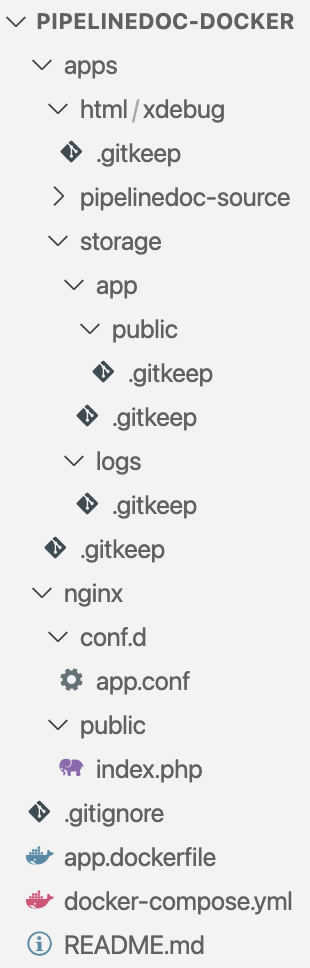
\includegraphics[width=0.30\textwidth]{img/pipelinedoc-docker-folders}
    \caption{La structure des dossiers du projet \Verb{pipelinedoc-docker}.}
    \label{fig:pipelinedoc-docker-folders}
\end{wrapfigure}

Le second projet, baptisé \Verb|pipelinedoc-source|, renferme le code source de l'API Pipeline documentaire. Ce dernier devra être cloné dans le dossier approprié au sein du projet \Verb|pipelinedoc-docker|. Cette étape est primordiale pour établir la connexion entre l'infrastructure Docker mise en place et le code de l'API à développer.

Les fichiers \Verb|app.dockerfile|, \Verb|docker-compose.yml| et le fichier de configuration Nginx sont essentiellement les mêmes que les fichiers présentés pour la production (Code source~\ref{code:dockerfile-prod}, page~\pageref{code:dockerfile-prod}; Code source~\ref{code:docker-compose-prod}, page~\pageref{code:docker-compose-prod}; Code source~\ref{code:nginx-conf-prod}, page~\pageref{code:nginx-conf-prod}). Cependant, bien qu'ils soient plus simples, ils ne contiennent pas toutes les instructions présentes dans ces fichiers.

Dès que les deux projets sont clonés, les conteneurs Docker peuvent être démarrés avec la commande suivante : \Verb|docker compose up|. Ensuite, le développeur doit créer le fichier \Verb|.env| pour le projet, contenant toutes les variables environnementales nécessaires, telles que les détails des connexions à la base de données, les URL et les jetons vers d'autres services, ainsi que d'autres paramètres de configuration. L'étape suivante consiste à installer les dépendances avec la commande \Verb|composer install| et à les mettre à jour avec la commande \Verb|composer update|. Ces commandes utilisent le fichier \Verb|composer.json| pour installer et mettre à jour les dépendances répertoriées avec leurs numéros de version. Ce projet inclut non seulement des dépendances publiques, mais également des dépendances développées et maintenues par l'entreprise dans son propre dépôt privé. Ces paquets privés sont ce que l'on appelle les \foreignquote{french}{cores}, comme nous l'avons mentionné précédemment (Figure~\ref{fig:architecture}, page~\pageref{fig:architecture}; Sous-section~\ref{subsec:cores}, page~\pageref{subsec:cores}).

Il reste encore trois petites étapes pour installer et démarrer complètement le projet : il faut lancer la commande \Verb|php artisan migrate:install|\footnote{Artisan est l'outil de ligne de commande intégré de Laravel, permettant d'effectuer diverses tâches liées au développement et à la gestion de projets Laravel.} pour créer la table \Verb|migrations| dans la base de données. Ensuite, il faut exécuter la commande \Verb|php artisan migrate| pour créer les tables nécessaires au projet, qui sont définies dans les fichiers de migration situés dans le dossier \Verb|database/migrations| du projet Laravel. Enfin, il faut utiliser la commande \Verb|php artisan queue:listen|\footnote{Ces commandes doivent bien sûr être exécutées dans le conteneur de l'application et à partir de son dossier racine.} pour démarrer la file d'attente de Laravel. À ce stade, le système est prêt à importer des fichiers et à exécuter ses autres fonctionnalités. Dans les lignes qui suivent, j'examinerai un peu plus en détail les fichiers de migration qui définissent la structure des tables de la base de données nécessaires au projet.